
\begin{figure}
    \centering
    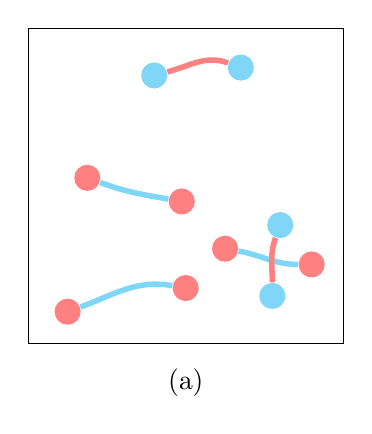
\begin{tikzpicture}
      \draw (0,0) rectangle (4,4);
      \node[circle, fill=red!50, minimum size=4] (N1) at (0.5,0.4) {};
      \node[circle, fill=red!50, minimum size=4] (N2) at (2,0.7) {};
      \node[circle, fill=red!50, minimum size=4] (N3) at (2.5,1.2) {};
      \node[circle, fill=red!50, minimum size=4] (N4) at (3.6,1) {};
      \node[circle, fill=red!50, minimum size=4] (N5) at (0.75,2.1) {};
      \node[circle, fill=red!50, minimum size=4] (N6) at (1.95,1.8) {};
      \node[circle, fill=cyan!50, minimum size=4] (N7) at (1.6, 3.4) {};
      \node[circle, fill=cyan!50, minimum size=4] (N8) at (2.7, 3.5) {};
      \node[circle, fill=cyan!50, minimum size=4] (N9) at (3.2, 1.5) {};
      \node[circle, fill=cyan!50, minimum size=4] (N10) at (3.1, 0.6) {};
      \draw[cyan!50, line width = 2] (N1) to[in=170, out=20] (N2);
      \draw[cyan!50, line width = 2] (N3) to[in=180, out=-10] (N4);
      \draw[cyan!50, line width = 2] (N5) to[in=170, out=-20] (N6);
      \draw[red!50, line width = 2] (N7) to[in=160, out=15] (N8);
      \draw[red!50, line width = 2] (N9) to[in=90, out=250] (N10);
      \node at (2, -.5) {(a)};
    \end{tikzpicture}
    \hspace{1cm}
    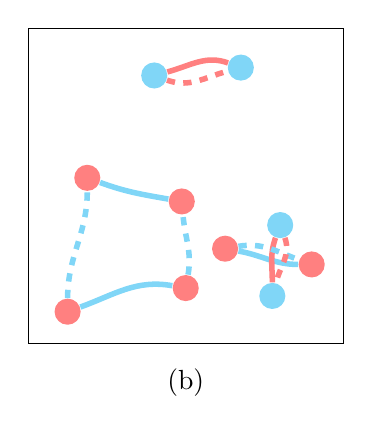
\begin{tikzpicture}
      \draw (0,0) rectangle (4,4);
      \node[circle, fill=red!50, minimum size=4] (N1) at (0.5,0.4) {};
      \node[circle, fill=red!50, minimum size=4] (N2) at (2,0.7) {};
      \node[circle, fill=red!50, minimum size=4] (N3) at (2.5,1.2) {};
      \node[circle, fill=red!50, minimum size=4] (N4) at (3.6,1) {};
      \node[circle, fill=red!50, minimum size=4] (N5) at (0.75,2.1) {};
      \node[circle, fill=red!50, minimum size=4] (N6) at (1.95,1.8) {};
      \node[circle, fill=cyan!50, minimum size=4] (N7) at (1.6, 3.4) {};
      \node[circle, fill=cyan!50, minimum size=4] (N8) at (2.7, 3.5) {};
      \node[circle, fill=cyan!50, minimum size=4] (N9) at (3.2, 1.5) {};
      \node[circle, fill=cyan!50, minimum size=4] (N10) at (3.1, 0.6) {};
      \draw[cyan!50, line width=2] (N1) to[in=170, out=20] (N2);
      \draw[cyan!50, line width=2] (N3) to[in=180, out=-10] (N4);
      \draw[cyan!50, line width=2] (N5) to[in=170, out=-20] (N6);
      \draw[red!50, line width=2] (N7) to[in=160, out=15] (N8);
      \draw[red!50, line width=2] (N9) to[in=90, out=250] (N10);
      \draw[cyan!50, dashed, line width=2] (N1) to[out=90, in=270] (N5);
      \draw[cyan!50, dashed, line width=2] (N2) to[out=80, in=275] (N6);
      \draw[cyan!50, dashed, line width=2] (N3) to[out=10, in=160] (N4);
      \draw[red!50, dashed, line width=2] (N7) to[out=-20, in=195] (N8);
      \draw[red!50, dashed, line width=2] (N9) to[out=290, in=75] (N10);
      \node at (2, -.5) {(b)};
    \end{tikzpicture}
    \hspace{1cm}
    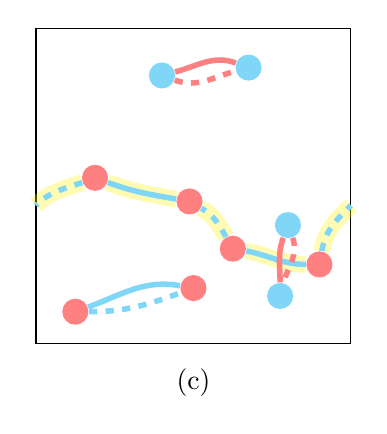
\begin{tikzpicture}
      \draw (0,0) rectangle (4,4);
      \node[circle, fill=red!50, minimum size=4] (N1) at (0.5,0.4) {};
      \node[circle, fill=red!50, minimum size=4] (N2) at (2,0.7) {};
      \node[circle, fill=red!50, minimum size=4] (N3) at (2.5,1.2) {};
      \node[circle, fill=red!50, minimum size=4] (N4) at (3.6,1) {};
      \node[circle, fill=red!50, minimum size=4] (N5) at (0.75,2.1) {};
      \node[circle, fill=red!50, minimum size=4] (N6) at (1.95,1.8) {};
      \node[circle, fill=cyan!50, minimum size=4] (N7) at (1.6, 3.4) {};
      \node[circle, fill=cyan!50, minimum size=4] (N8) at (2.7, 3.5) {};
      \node[circle, fill=cyan!50, minimum size=4] (N9) at (3.2, 1.5) {};
      \node[circle, fill=cyan!50, minimum size=4] (N10) at (3.1, 0.6) {};
      \draw[yellow, line width=6, opacity=.3] (N3) to[in=180, out=-10] (N4);
      \draw[yellow, line width=6, opacity=.3] (N5) to[in=170, out=-20] (N6);
      \draw[yellow, line width=6, opacity=.3] (N3) to[out=120, in=-30] (N6);
      \draw[yellow, line width=6, opacity=.3] (N5) to[out=200, in=45] (0, 1.75);
      \draw[yellow, line width=6, opacity=.3] (N4) to[out=80, in=225] (4, 1.75);
      \draw[cyan!50, line width=2] (N1) to[in=170, out=20] (N2);
      \draw[cyan!50, line width=2] (N3) to[in=180, out=-10] (N4);
      \draw[cyan!50, line width=2] (N5) to[in=170, out=-20] (N6);
      \draw[red!50, line width=2] (N7) to[in=160, out=15] (N8);
      \draw[red!50, line width=2] (N9) to[in=90, out=250] (N10);
      \draw[cyan!50, dashed, line width=2] (N1) to[out=0, in=200] (N2);
      \draw[cyan!50, dashed, line width=2] (N3) to[out=120, in=-30] (N6);
      \draw[cyan!50, dashed, line width=2] (N5) to[out=200, in=45] (0, 1.75);
      \draw[cyan!50, dashed, line width=2] (N4) to[out=80, in=225] (4, 1.75);
      \draw[red!50, dashed, line width=2] (N7) to[out=-20, in=195] (N8);
      \draw[red!50, dashed, line width=2] (N9) to[out=290, in=75] (N10);
      \node at (2, -.5) {(c)};
    \end{tikzpicture}
    \caption{The quasiparticle picture of stabilizer measurements. Anticommuting stabilizers behave as anyons (circles), where a chain of errors (lines) creates a pair of anyons. Figure (b) shows a successful decoding of (a). Figure (c) shows a pairing that resulted in a correction operator that is in a different class as the error operator, which acquires a logical error. (Figure inspired by \cite{naomi})}\label{fig:quasiparticle}
  \end{figure}
  